\chapter{OTFVis: MATSim's Open-Source Visualizer}
\label{ch:otfvis}
% ##################################################################################################################

\hfill \textbf{Author:} David Strippgen

\begin{center} 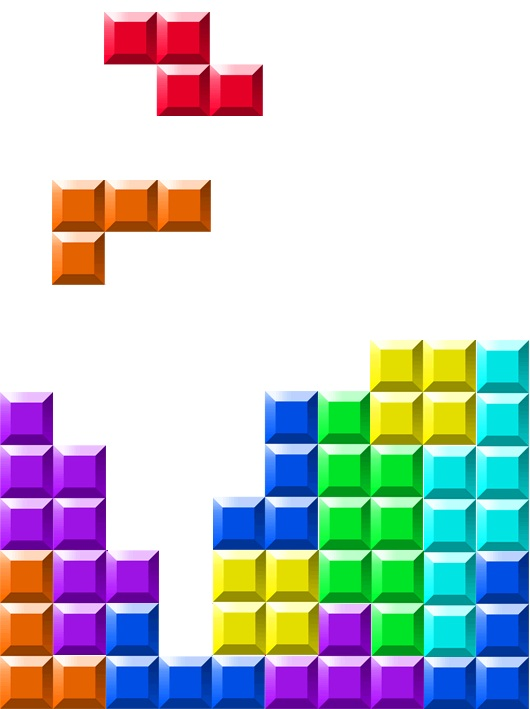
\includegraphics[width=0.25\textwidth, angle=0]{frontmatter/figures/MATSimBook} \end{center}

\createStandardInformationBasic{\url{http://matsim.org/javadoc} $\to$ contrib $\to$ otfvis}{Run \lstinline|org.matsim.contrib.otfvis.RunOTFVis| class}{No further configuration required.}{\citet[][]{Strippgen_PhDThesis_2009}}

% ##################################################################################################################
\gls{otfvis} is the open-source alternative to \gls{senozon} \gls{via}. 
\gls{otfvis} is able to visualize results during runtime of a \gls{matsim} run. 
It is available as a \gls{contribution}. 
It is implemented in \gls{java}; to make use of sophisticated visualization of the OpenGL framework, it is also heavily based on jogl. 
%This requires a couple of user actions to get jogl running on his specific platform. \ah{not true anymore}

% ################################################################################################################

\url{urn:nbn:de:kobv:83-opus-23640}





